\paragraph{Bonus - Esquema de atenuação/desligamento do sinal persistentemente excitante}

Para uma planta genérica onde o sinal introduzido é persistentemente excitante e da forma $u_{(t)}= \sum  \varepsilon_iKsin(w_it) + u_0$ onde as escolhas de $\varepsilon_i$ são valores constantes e K é uma fração do nível de referência $u_0$,transformamos os valores de $\varepsilon_i$ em variáveis com o valor limitado entre 0 e 1 e determinados pela equação $\varepsilon_i = \frac{\dot{\hat{\theta^{T}}}Q\dot{\hat{\theta}}}{1 +\dot{\hat{\theta^{T}}}Q\dot{\hat{\theta}}}$, de forma que a medida que a atualização dos parâmetros se torna menor, a amplitude do sinal persistentemente excitante vai se tornando menor até zerar.

Testamos esta ideia a partir da planta de ordem 1 usada na questão 2, com os valores $R=1.2\Omega;L = 0.01H$. Obtivemos um comportamento da função $\varepsilon_1$ com variações abruptas, de forma a evitar desligamentos e religamentos repetidos do sinal, resolvemos filtrar $\varepsilon_1$ através de um filtro passa baixa. Usamos um sinal da forma $u_{(t)}=100\varepsilon_1\sin(20\pi t) + 100$ para fazer a estimação. Os resultados obtidos foram os seguintes: 

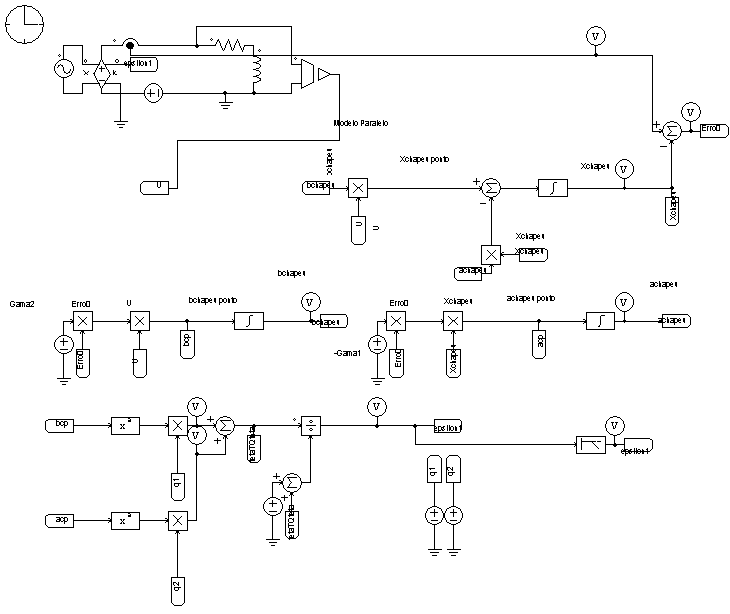
\includegraphics[width = 14 cm, height = 8 cm]{./pic/BonusMontagem.png}

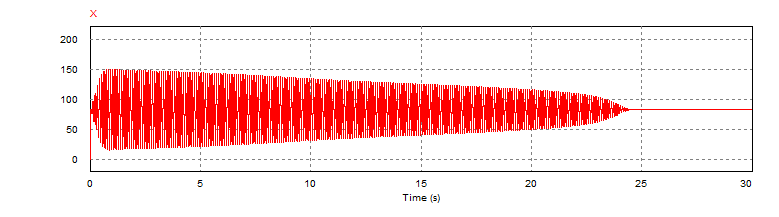
\includegraphics[width = 14 cm, height = 8 cm]{./pic/BonusX.png}

\includegraphics[width = 14 cm, height = 8 cm]{./pic/BonusXchapeu.png}

\includegraphics[width = 14 cm, height = 8 cm]{./pic/BonusEpsilon1.png}

Aqui podemos notar o comportamento de Epsilon1 como sendo um sinal que varia abruptamente, já que os valores da atualização dos parâmetros não são constantes é natural que isto aconteça. Portanto para evitar introduzir estas variações abruptas na planta escolhemos filtrar o sinal através de um filtro passa baixa de segunda ordem com frequência de corte $f_c = 1Hz$.

\includegraphics[width = 14 cm, height = 8 cm]{./pic/BonusEpsilon1Filtered.png}

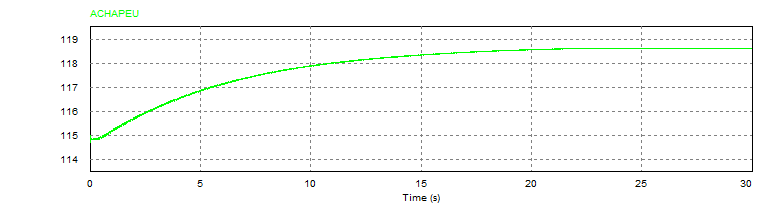
\includegraphics[width = 14 cm, height = 8 cm]{./pic/BonusTeta1.png}

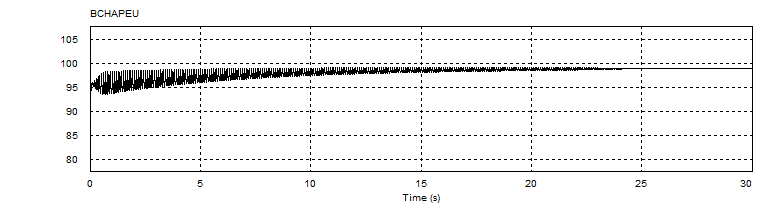
\includegraphics[width = 14 cm, height = 8 cm]{./pic/BonusTeta2.png}

E vemos que o sinal P.E desliga após os valores dos parâmetros se aproximarem suficientemente dos corretos.

\includegraphics[width = 14 cm, height = 8 cm]{./pic/BonusEsaida.png}

E também que a introdução deste método de atenuação do sinal P.E não afetou a convergência da saída do modelo para a saída da planta.